\section{Use cases}

%TODO
\begin{figure}[ht]
	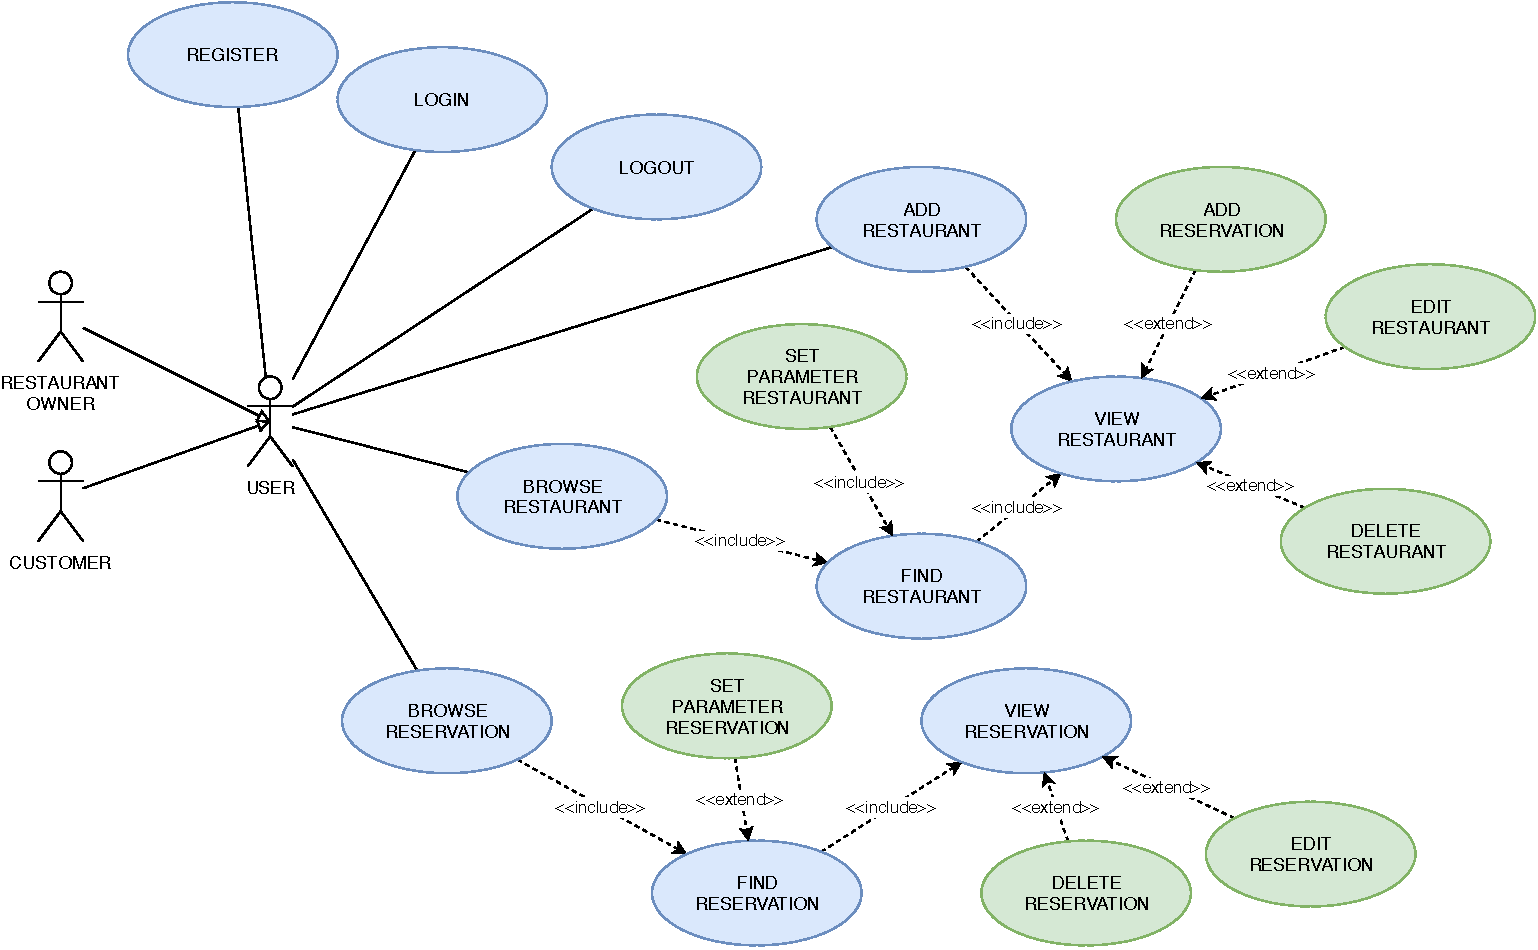
\includegraphics[width=\textwidth]{usecases}
	\caption{Use cases diagram.}
	\label{fig:usecases}
\end{figure}

\begin{itemize}
	\item[Registration] The first time a user uses the application  he/she
		will be asked to register himself/herself, providing an username
		and a password, and specifying which type of user he/she is
		(customer or restaurant owner).
	\item[Login] (Require Registration) A User (customer or restaurant
		owner), will provide his credentials, the application will check
		if he/she is in the system and then will grant or deny the
		access, depending on the result of the check.
	\item[Browse Restaurant] (Require Login) The list of all available
		restaurant, with description, genre, price, and number of seats
		available. The list is provided to customers from which they
		can choose the restaurant to book. Furthermore a user can filter
		the element of the list specifying the city.
	\item[Browse Reservation] (Require Login) The list of all the
		reservations made. For the customers, it is the list of their
		reservations made for different restaurants. For the restaurant
		owners, this is the list of reservations made by customers in
		their restaurants. Only reservations for the present day and
		future days are shown to the user.
	\item[Add Restaurant] (Require Login) When creating a "restaurant owner"
		type user, a restaurant is created.
	\item [Delete Restaurant] (Require Login) An owner can delete a
		restaurant, after this operation the owner account will not be
		deleted, but it will be a Customer account.\footnote{This
		functionality is only implemented into the command line
		interface version of the program}
	\item[Edit Restaurant] (Require Login) a restaurant owner is able to
		modify his/her restaurant.
	\item[Add Reservation] (Require Login) Customers can make a reservation
		at one of the available restaurants.
	\item[Delete Reservation] (Require Login) Customers can delete a
		reservation made in the past.
	\item[Edit Reservation] (Require Login) Customers can modify a
		reservation made in the past.
\end{itemize}
